\documentclass{article}
\synctex=1
\usepackage{arxiv}
\usepackage{graphicx}
\usepackage{caption}
\usepackage{tikz}
\usepackage{svg}
\usepackage[utf8]{inputenc} % allow utf-8 input
\usepackage[T1]{fontenc}    % use 8-bit T1 fonts
\usepackage{hyperref}       % hyperlinks
\usepackage{url}            % simple URL typesetting
\usepackage{booktabs}       % professional-quality tables
\usepackage{amsmath, amssymb, amsfonts}       % blackboard math symbols
\usepackage{nicefrac}       % compact symbols for 1/2, etc.
\usepackage{microtype}      % microtypography
\usepackage{cleveref}       % smart cross-referencing
\usepackage{lipsum}         % Can be removed after putting your text content
\usepackage{graphicx}
\usepackage{caption}
\usepackage{subcaption}
%\usepackage{natbib}
%\usepackage[backend=biber,style=apa,apabackref=true,uniquelist=false]{biblatex}
\usepackage[backend=biber,style=apa,backref=true,uniquelist=false]{biblatex}
%\usepackage[backend=biber,style=numeric,uniquelist=false]{biblatex}
%\usepackage{biblatex}
\usepackage{doi}
\usepackage{svg}
\usepackage[toc,page]{appendix}
%\usepackage{import}

\usetikzlibrary{shapes,arrows,positioning}


\graphicspath{images/}
\title{Electric vehicle energy optimization system --- A case study for applications of deep reinforcement learning in the real world}


% Here you can change the date presented in the paper title
%\date{September 9, 1985}
% Or remove it
%\date{}

\newif\ifuniqueAffiliation
% Comment to use multiple affiliations variant of author block
\uniqueAffiliationtrue

\ifuniqueAffiliation % Standard variant of author block
\author{ \href{https://orcid.org/0009-0003-0705-2612}{\includegraphics[scale=0.06]{orcid.pdf}\hspace{1mm}Binjian Xin}\thanks{} \\
	Shanghai\\
	\texttt{binjian.xin@gmail.com} \\
	%% examples of more authors
	%% \AND
	%% Coauthor \\
	%% Affiliation \\
	%% Address \\
	%% \texttt{email} \\
	%% \And
	%% Coauthor \\
	%% Affiliation \\
	%% Address \\
	%% \texttt{email} \\
	%% \And
	%% Coauthor \\
	%% Affiliation \\
	%% Address \\
	%% \texttt{email} \\
}
\else
% Multiple affiliations variant of author block
\usepackage{authblk}
\renewcommand\Authfont{\bfseries}
\setlength{\affilsep}{0em}
% box is needed for correct spacing with authblk
\newbox{\orcid}\sbox{\orcid}{\includegraphics[scale=0.06]{orcid.pdf}}
\author[1]{%
	\href{https://orcid.org/0009-0003-0705-2612}{\usebox{\orcid}\hspace{1mm}Binjian Xin\thanks{\texttt{binjian.xin@gmail.com}}}%
}
\affil[1]{}
\fi

% Uncomment to override  the `A preprint' in the header
%\renewcommand{\headeright}{Technical Report}
%\renewcommand{\undertitle}{Technical Report}
\renewcommand{\shorttitle}{\textit{arXiv} Template}

%%% Add PDF metadata to help others organize their l ibrary
%%% Once the PDF is generated, you can check the metadata with
%%% $ pdfinfo template.pdf
\hypersetup{
pdftitle={Electric Vehicle Optimizaiton System},
pdfsubject={q-bio.NC, q-bio.QM},
pdfauthor={Binjian Xin},
pdfkeywords={Deep Reinforcement Learning, Electric Vehicle, Time Series},
}


%\bibliography{rl.bib}  %%% Uncomment this line and comment out the ``thebibliography'' section below to use the external .bib file (using bibtex) .
%\addbibresource{rl.bib,veos.bib}
%\bibliography{rl,veos}
%\bibliography{references.bib}
\addbibresource{rl.bib}
\addbibresource{veos.bib}

\begin{document}
\maketitle

\begin{abstract}
	We present the application of deep reinforcement learning in the optimization of energy efficiency of driving an electric vehicle. The optimziation is modeled as Markov Decision Process and the design choice of the state, action and reward is provided. We set up a flexible data pipeline for capturing, processing, storing and sampling time sequences which enables both online and offline reinforcement learning. The training and inferring setup of the agent are provided with respect to the practical technicalities. Our system is scalable by leveraging the cloud infrucstructure therefore is capable of handling a massive fleet in scope of the application asynchronously in training and infering deployment. We observe the manifest increase of the energy efficiency on the real road condition within a short time range of online training. We assume the driver behavior is stationary and montior the driving style during training and give an analysis of the interaction between the human driver and the agent. We verify the transferability and multimodality of the trained model on different road conditions and give a review of safety, sample efficiency, data synchronicity of the system concerning the applications of deep reinforcement learning in the real world. Solutions are provided for solving partial observability, long-term stragtegy and efficient training of ragged episode length by leveraging sequential models. Deployment of reward-driven learning methods can promote the industry to leverage abundant available online or offline domain data and interfaces to achieve continuous and dynamic optimization in many complex industrial processes which require the large capacity of deep neural networks.
\end{abstract}

% keywords can be removed
\keywords{deep reinforcement learning \and electric vehicle \and time series \and dataflow}

\section{Introduction}\label{sec:intro}

Drivers with diverse driving experience tend to have quite different fuel or electricity consumption on the same vehicle and the same driving route. The general common sense is that the driving styles, i.e., how drivers operate the vehicle through acceleration and brake, have an impact on the vehicle energy consumption. We would expect there exists an experienced driver with a specific driving style can handle various road conditions to achieve the optimal energy efficiency. This leads us to the assumption that if we could apply an agent which observe the driving dynamics and adjusts the driving operation, we could reduce the energy consumption. If we choose the right observation and action, we could optimize the energy consumption online or offline for driving the vehicle with a general paradigm based on learning methods so that we can leverage a large mount of easily available driving data.

Nevertheless, the application of deep reinforcement learning in the real world is generally difficult \parencite{Irpan_2018}. The main reasons include the sample inefficiency, reward shaping challenge, local optima, overfitting to rare patterns, unstable training, hyperparameter sensitivity. Most known successful applications of deep reinforcement learning can be found in games \parencite{mnih13:_playin_atari_deep_reinf_learn}, \parencite{DBLP:journals/nature/SilverHMGSDSAPL16}, \parencite{DBLP:conf/ijcai/BrownS17}, \parencite{openai19:_dota_large_scale_deep_reinf_learn}, \parencite{bakhtin22:_Human_level_diplomacy_cicero}, where the system dynamics are deterministic or closely deterministic.
If the system dynamics is deterministic or very well known and a good simulation is available, then an enormous amount of samples can be generated for training. Furthermore for games specifically, self-play can be used for learning \parencite{Silver_2018}.

In recent years, robotics is the domain with growing successful deployment of deep reinforcement learning in the real world, particularly in manipulation, grasping and legged locomotion. Diverse techniques are used. Usually simulation is leveraged to have a good model for transfer learning in the real world. In particular privileged information of the system dynamics is used to have dedicated modules to explicitly deal with environment changes \parencite{kumar21:_rma}, to learn the alignment of proprioception with exteroception \parencite{Miki_2022}, or to just use a specialized initialization strategy, randomized physical parameters and intentional delay in simulation for efficient exploration \parencite{Song_2023}. Furthermore, \parencite{Hoeller_2024} focuses on limited skill sets to have a modular model structure to increase the learning efficiency. \parencite{smith23:_grow_your_limit} constrains the policy in a principled way to the familiar system dynamics to increase the learning efficiency in the real world. \parencite{wu22:_daydr} leverages the world model and efficient sequential latent encoding of the system dynamics. Overall robotics learning tends to use more imitation learning and utilize offline data, as it's still hard to search for the generic reinforcement learning and extra pre-training and supervised fine-tuning is cheaper \parencite{Irpan_2024}.

In the automotive industry, the most evident applicaion would be autonomous driving. But there's no available public work of autonomous driving in the real world that's based on deep reinforcement learning framework in a principled way. More attention is paid to leveraging simulation to generate sufficient training samples or using prior knowledge in pretrained foundational models and scaling up.

In general, there's no generic end-to-end deep reinforcement learning method for real world applications, but a paradigm to combine deep reinforcement learning with domain specific techniques to alleviate the aforementioned challenges. As each problem in the real world have its specific prior information and exploitable inductive biases, it's only natural to exploit them in an engineering way.
ff
This paper gives an example that progress in real world applications can be achieved with deep reinforcement learning. While research concerns might be alleviated with design choices, the practical deployment should still comply with the basic requirements of the theories stringently without loss of validity. Eventually in long term, issues of multimodality and out-of-distribution matter in complex and very long time horizon. On the practical side, deployment of reward-driven learning methods can promote the industry to leverage abundant available online or offline domain data and interfaces to achieve continuous and dynamic optimization in many complex industrial processes which require the large capacity of deep neural networks and have the potential to help reshaping the industry into the data-driven paradigm.

\subsection{Related work}\label{sec:related}

Electric vehicles (EVs) have been growing in popularity in the automotive industry with sales increasing globally. The share of electric cars in total sales has increased from negligibly less than 0.1\% in 2010 to 14\% in 2022 \parencite{statista_2023}. The deployment of EVs is largely due to the rising fuel economy standards and the required reduction in greenhouse gas emissions, which leads to the increasing complexity of powertrains in the form of additional actuators and control systems. The energy efficiency of EVs has been the focus of powertrain electrification. In \parencite{Egan_2023} an overview of the reinforcement learning methods applied in powertrain controllers in hybrid electric vehicles (HEVs), fuel cell electric vehicles (FCEVs), plug-in hybrid electric vehicles (PHEVs) is given. They reviewed the state, action space and the reward function of their design choices.

For example, \parencite{Wang_2020} exploits the physical models of extended range electric electric vehciles (EREVs) in the investigation so that the chosen state consists of the traveled distance and time, fuel use and the GPS coordinates of the vehicle and in particular the ``energy compensated expected trip distance'' which by their definition is the expected total trip distance multiplied by a ratio of trip energy intensity and the expected one. The chosen action is the range of the constructed state. The reward function is designed as weighted sum of the penaltes of internal combustion engine (ICE) operation, low state of charge (SOC), change of the constructed state and a specific terminal state. In \parencite{Hou_2022} the state is defined as the power demand and SOC, the action is the fuel cell power, while the reward is a weighted sum of the change rate of the instantaneous hydrogen consumption, a qudratic poloynomial of the battery power with cooefficients containing open-circuit voltage, cell capacity and battery internal resistance in order to reduce unnecessary energy storation while keep the action feasiblity of the electric motor and the internal combustion engine (ICE). Similarly, \parencite{Hu_2018} selects for HEVs the total required torque and SOC as state and the output torque of ICE as action which is equivalent to the power-split of HEV between the electric motor and ICE, while the reward is defined as the reciprocal of instantaneous fuel consumption of the ICE conditioned on the range of itself and the instantaneous SOC\@.

It can be seen that these methods exploit the domain specific knowledge for each of the vehicle model under investigation to select the state and action. The constructed and estimated expectation state signals which are not directly measured contain further biases and noise. Besides, the measureable state signals in those applications require specific sensors or processing and are thus expensive to acquire. Furthermore, it should be noted that even the SOC cannot be directly measured in real time while the vehicle is driving so it's estimated from the measured voltage and a lookup table acquired by calibration. The selected actions serve their specific objective domains and therefore cannot be generalized to other vehicle models. The reward shaping in those applications are never the energy consumption directly, since the objective is to optimize the co-operation of eletric motor and ICE for HEV\@. It's usually a heuristic mixture of electricity and fuel consumption with constraints which are required to regularized the system behavior but in general detrimental to the optimization performance. The weights in the reward brings extra hyperparameters which is sensitive to the system performance and difficult to analyse.

The review of the applications of deep reinforcement learning in EVs makes us wonder whether we can use the energy consumption directly as reward, while taking observation directly from the vehicle dynamics and driver behavior. The objective would not be the optimization of the co-operation of the mixed powertrain components, but the optimization of overall powertrain dynamic behavior conditioned on the road environment and driver operation. We'd call such a system ``Electric Vehcicle Energy Optimization System'' (EVEOS). Such a system would be generic and applicable for any type of EVs since all the required observations, actions and rewards would be available and easily measureable. The challenge is to learn the complex system dynamics of driving in the real world condition.

It shoud be noted that the method would applicable for regular ICE vehicles as well. We experiment on a BEV, since it has a simplistic yet powerful electric powertrain. The electric motor has a much faster torque response than ICE, therefore the measurements are more precise and have better real-time performance which is crucial to guarantee the causality of actions, states and rewards.

Empirically, the optimization space of the driving operation comes from the way to adjust the vehicle speed by acceleration or deceleration to reach the target position with the target speed. Usually a smooth speed transition is better than abrupt acceleration or braking which causes large currents in the electric motor and results in more electricity consumption. One particular feature of EVs is regenerative braking system (RBS) \parencite{enwiki:1228286642}, which lets the vehicle recapture energy from momentum by running the electric motor in reverse to recharge the battery. The regenrative braking system improves the energy efficiency and is now a standard part of many electrified vehicle including HEVs and BEVs. The parameters of the RBS are contained in the electironic control unit (ECU) of the vehicle powertrain controller which is called vehicle control units (VCU). Usually the RBS doesn't depend on road conditions or driver operations and is implicitly static. However, if we choose the action so that it can impact the RBS, under the EVEOS the RBS can be exploited by the agent like the other acceleration or braking strategies. We observe in the experiment that even without explicitly modeling the RBS behaviour in the system, the RBS is actively and legitmately exploited by the agent to reduce the energy consumption without any explicit built-in rules or modeling.

\section{Preliminary}\label{sec:intro:preliminary}

In order to increase the energy efficiency while driving, we consider the following structure in Fig. \ref{fig:Agent_Powertrain}. Without the agent and its connection to the input (observation) and the output (action), the parameters of the powertrain controller are kept static, the depicted process is a regular powertrain control with the driver in the loop. The driver controls the vehicle speed through acceleration and brake pedal while observing the road condition.

\tikzset{block/.style = {draw, fill=white, rectangle, minimum height=3em, minimum width=6em},
	input/.style = {coordinate},
	signal/.style = {circle, fill, inner sep=1pt},
	coord/.style = {coordinate},
	pinstyle/.style = {pin edge={<-,thin,black}}}

\begin{figure}[!h]
	\centering
	\scalebox{0.8}{
		\begin{tikzpicture}[auto, node distance=3cm,>=latex']

			\node [input, name=input] {};
			\node [block, right = 1cm of input] (driver) {Driver};
			\node [block, right of=driver, align=center] (pedals) {Accelerate \& \\ Brake Pedal};
			\node [signal, right=0.5cm of pedals] (psensor) {};
			\node [block, right= 0.5cm of psensor, align=center] (vcu) {Powertrain \\ Controller};
			\node [block, right of=vcu] (pt) {Powertrain};
			\node [signal, right=0.5cm of pt] (vasensor) {};
			\node [block, right= 0.5cm of vasensor] (vehicle) {vehicle};
			\node [signal, right of=vehicle] (output) {};
			\node [block, above = 1cm of vcu] (agent) {Agent};
			\node [coord, below = 1cm of vcu] (feedback) {feedback};

			\draw [->] (input) -- (driver);
			\draw [->] (driver) -- (pedals);
			\draw [-] (pedals) -- (psensor);
			\draw [->] (psensor) -- (vcu);
			\draw [->] (vcu) -- (pt);
			\draw [->] (pt) -- (vehicle);
			\draw [->] (vehicle) -- (output);
			\draw [->,thick] (output) |- node [above, pos=0.95] {$V$} (agent.20);
			\draw [->,thick] (vasensor) |- node [above, pos=0.85] {$U$, $I$} (agent.340);
			\draw [-] (output) |- (feedback);
			\draw [->,thick] (psensor) |- node [above, pos=0.6]{$A$,$B$} (agent);
			\draw [-] (feedback) -|  (input);
			\draw [->,thick] (agent) -- node [right, pos=0.6] {$\Delta T$}(vcu);
		\end{tikzpicture}
	}
	\caption{Add an agent to the conventional EV powertrain control loop.}
	\label{fig:Agent_Powertrain}
\end{figure}

When the agent is connected to the regular system as depicted, it will get the vehicle speed $V$, the driver's operation on the acceleration pedal $A$ and the brake pedal $B$ from the on-board sensors as its observation. $V, A, B$ is defined as the state of EVEOS system. In order to reduce the observation dimensionality, we take only the longitudinal control the vehicle, namely the electric powertrain into account, since the lateral operation through the steering wheel has far less impact on the energy consumption than the longitudinal control. The negative of the engergy consumption, which is the product of the voltage $U$ and the current $I$ from the sensors in powertrain, $U\cdot V$, when multiplied by a time constant, is directly taken as the instantaneous reward. Here we have the real reward. The action $\Delta T$ is chosen to be the change of torque request incrementally added onto the ``pedal map'' of the VCU\@.

\begin{figure}[ht]
	\centering
	\begin{subfigure}[b]{0.45\textwidth}
		\centering
		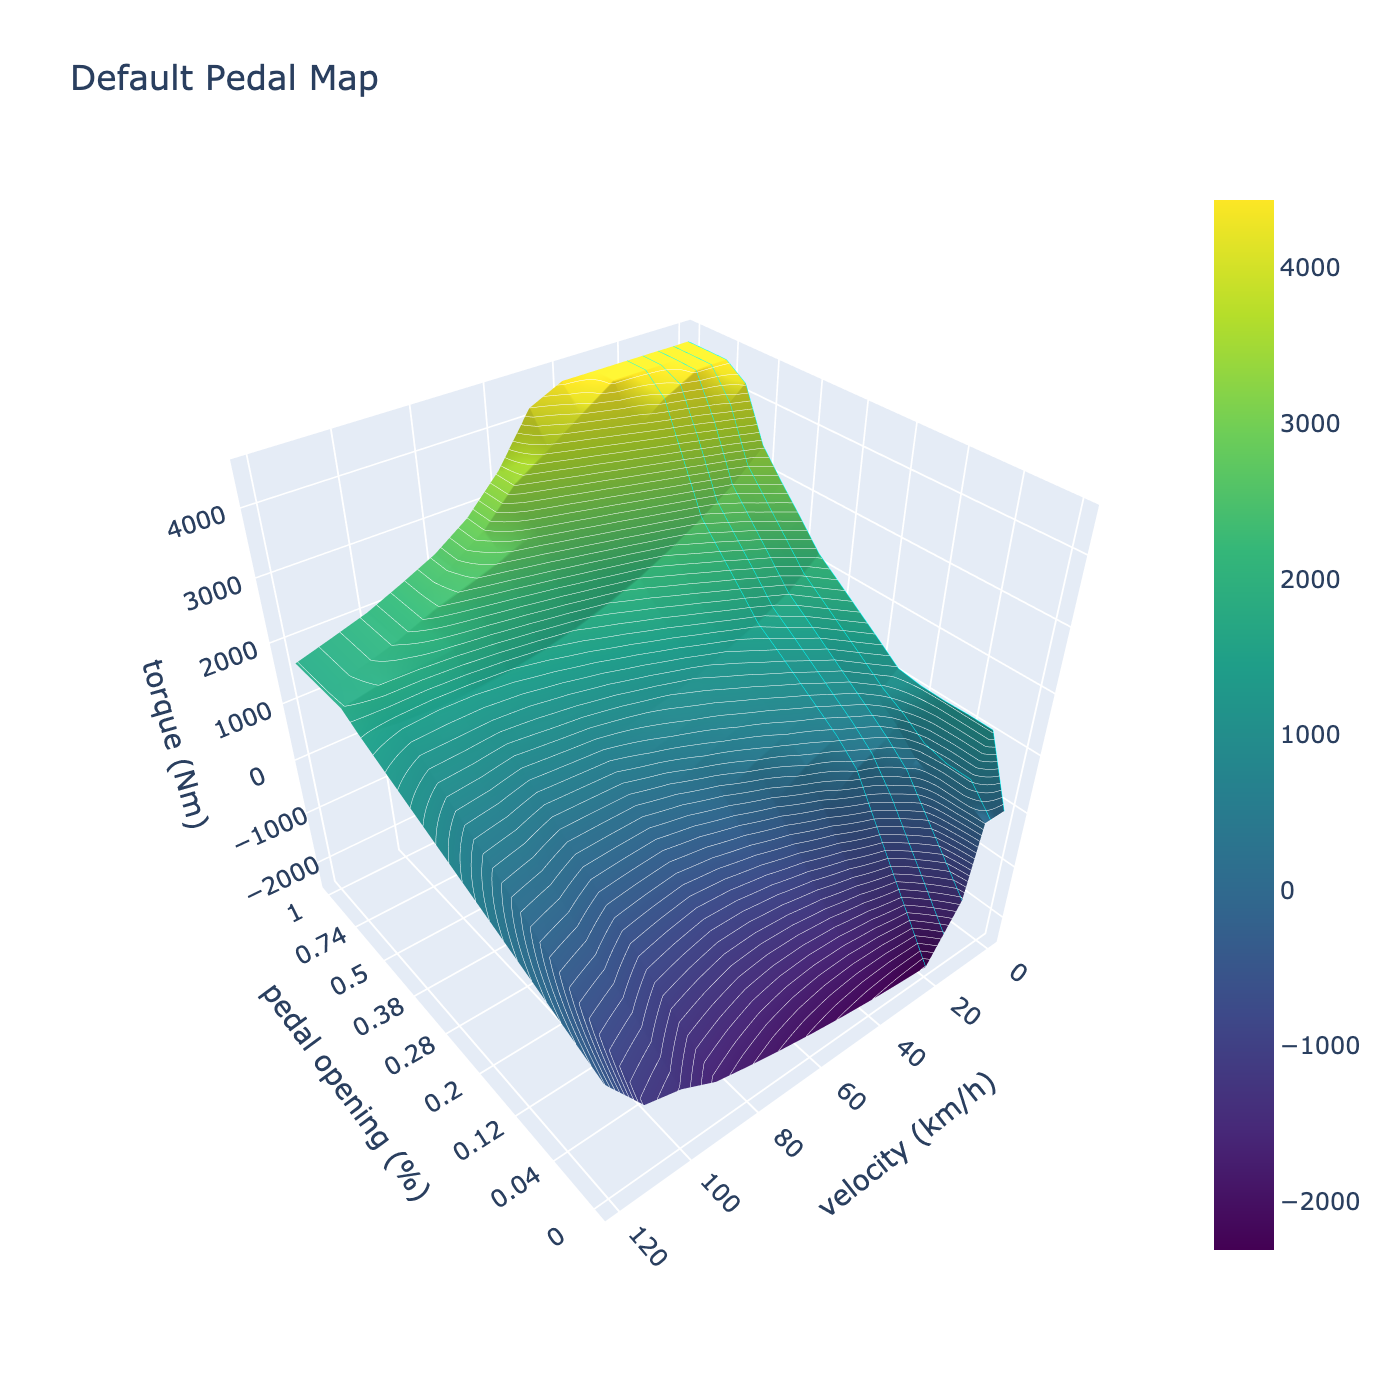
\includegraphics[width=\textwidth]{images/table_init.png}
		\caption{The ``Economic'' pedal map as the initial map}
		\label{fig:initial pedal map}
	\end{subfigure}
	\hfill
	\begin{subfigure}[b]{0.45\textwidth}
		\centering
		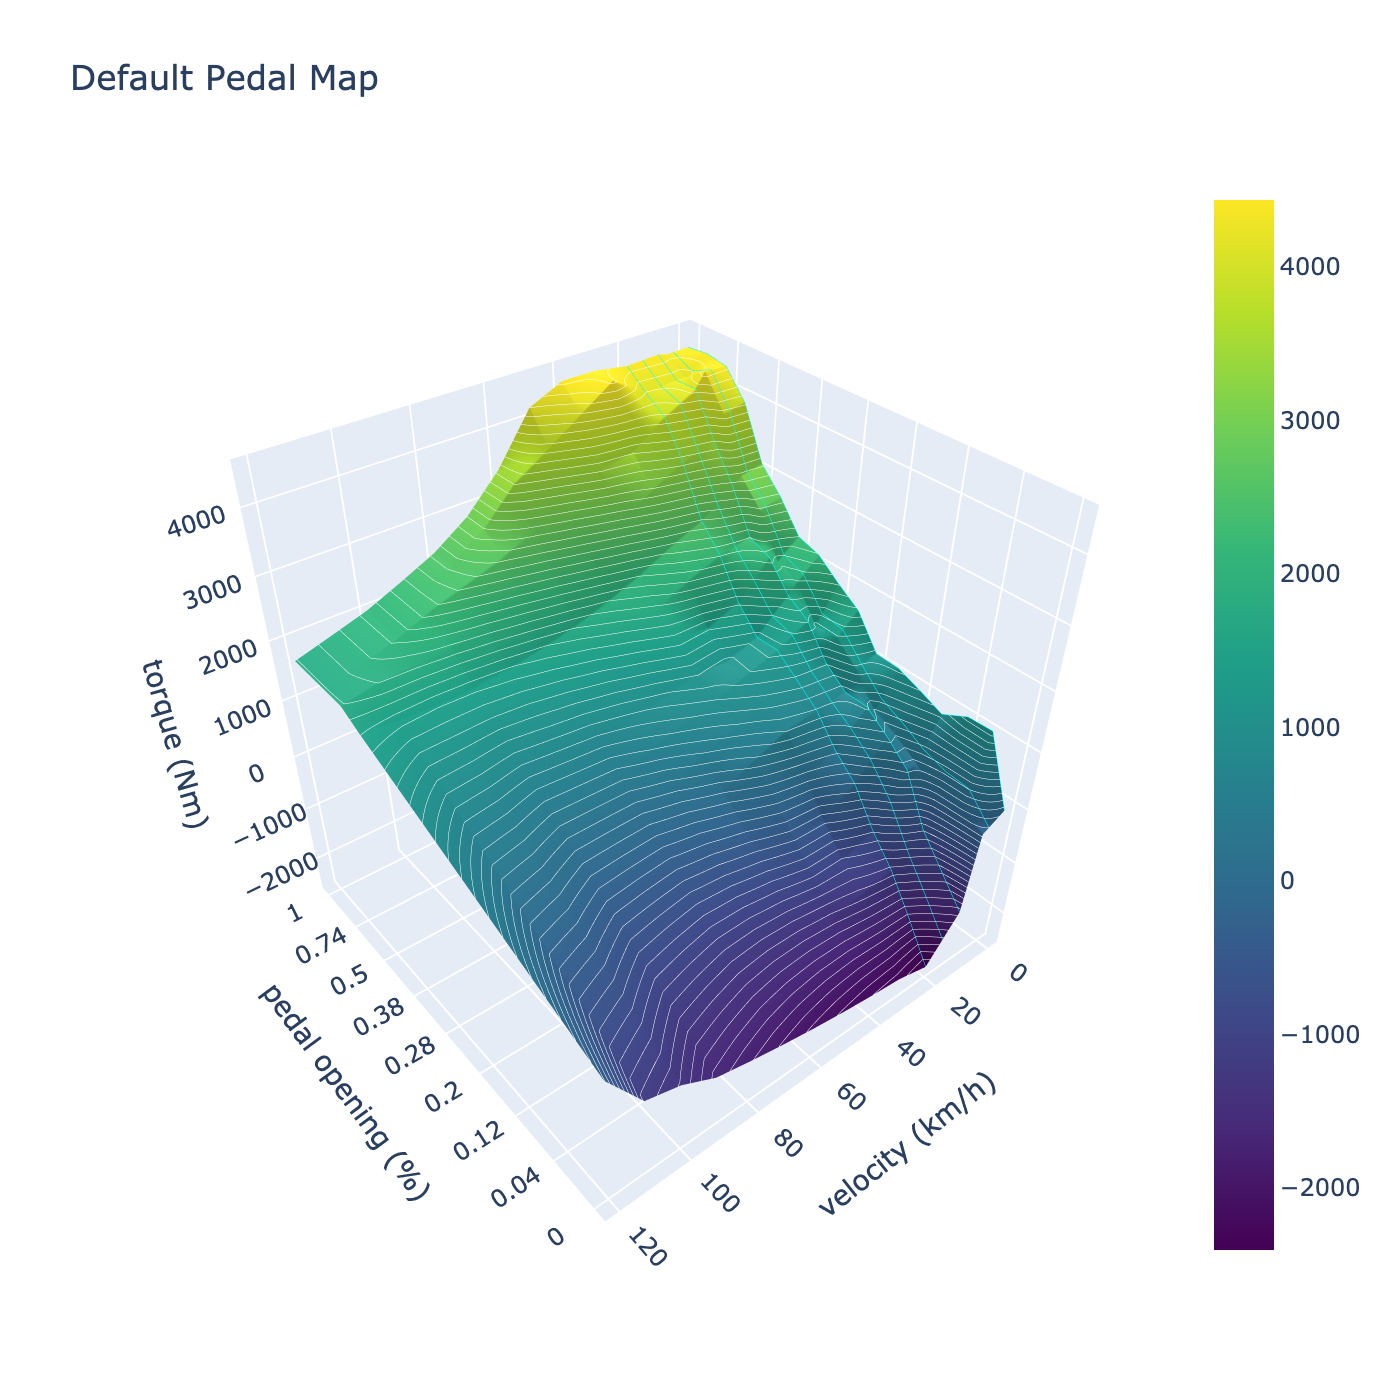
\includegraphics[width=\textwidth]{images/table_final.png}
		\caption{The dynamic pedal map}
		\label{fig:dynamic pedal map}
	\end{subfigure}
	\caption{\label{fig:pedal map} A pedal map is a 2d mapping table which outputs the torque request given a pedal opening under a certain vehicle speed. (a) The ``Economic'' pedal map is used as initial pedal map by the agent. (b) The pedal map is dynamically modified by the agent during driving conditioned on the vehicle speed and driver operation.}
\end{figure}

The pedal map is a two-dimensional table which gives the torque request to the electric motor for a given acceleration pedal opening under a certain vehicle speed. It's a static map for a regular powertrain controller, as depicted in Fig.\@\ref{fig:pedal map}. The requested torque, once exerted by the electric motor, is proportional to teh vehicle acceleration. It's usually acquired by vehicle calibration during the pre-development of the EV model. A calibration engineer will generate different pedal maps by testing drives on proving ground or real road and determine table items empirically and by experimental validation. The different pedal maps will correspond to different driving styles which are provided as features to the customers, such as ``Normal'', ``Sport'' or ``Economic''. The customers will choose a driving a pedal map through a vehicle HMI to match their driving style requirements. We select the ``Economic'' pedal map as the default initial pedal map for the agent and check how much the agent can further improve the energy efficiency. The pedal map increases monotonically with the acceleration pedal opening, while decreasing monotonically with the vehicle speed. The maximal torque request occurs when the vehicle starts off and the drive steps on the pedal with full throttle. The map region with low speed ($\leq10kmph$) and negligible pedal openings has the largest the negative torque request, which corresponds to motor in reverse, i.e.\ strong regenerative braking. These are all by design.

When the agent change the torque request a given range of vehicle speeds under a give pedal opening, the corresponding region of the pedal map will be changed by $\Delta T$. If the training occurs on a urban road, we can see the low speed region under 60 kmph is changed as depicted in Fig.\ref{fig:dynamic pedal map}. The resulting pedal map is the sum of the initial map and integration of the action up to the current moment. In our experiment the agent is allowed to change the items all over the map region, which allows implicitly the exploitation of the regenerative braking.

\section{Training}\label{sec:training}

Episode

\begin{figure}
	\begin{minipage}[b]{0.45\linewidth}
		\centering
		\begin{tabular}{c c c c c}
			\toprule
			$t$     & $s_{t}$                               & $a_t$              & $r_t$                    & $s'_t$                                   \\
			\cmidrule(r){1-1} \cmidrule(r){2-4} \cmidrule{5-5}
			1       & $V_1$, $A_1$, $B_1$                   & $\Delta T_{1}$     & $U_{1}$, $I_{1}$         & $V'_1$, $A'_1$, $B'_1$                   \\
			\ldots  & \ldots                                & \ldots             & \ldots                   & \ldots                                   \\
			$i_{1}$ & $V_{i_{1}}$, $A_{i_{1}}$, $B_{i_{1}}$ & $\Delta T_{i_{1}}$ & $U_{i_{1}}$, $I_{i_{1}}$ & $V'_{i_{1}}$, $A'_{i_{1}}$, $B'_{i_{1}}$ \\
			        & \ldots                                & \ldots             & \ldots                   & \ldots                                   \\
			$i_{l}$ & $V_{i_{l}}$, $A_{i_l}$, $B_{i_l}$     & $\Delta T_{i_{l}}$ & $U_{i_{l}}$, $I_{i_{l}}$ & $V'_{i_{l}}$, $A'_{i_{l}}$, $B'_{i_{l}}$ \\
			\ldots  & \ldots                                & \ldots             & \ldots                   & \ldots                                   \\
			K       & $V_K$, $A_K$, $B_K$                   & $\Delta T_{K}$     & $U_K$, $I_K$             & $V'_K$, $A'_K$, $B'_K$                   \\
			\bottomrule
		\end{tabular}
		\captionof{table}{\label{tab:quadruple}Sample table}
	\end{minipage}\hfill
	\begin{minipage}[b]{0.45\linewidth}
		\centering
		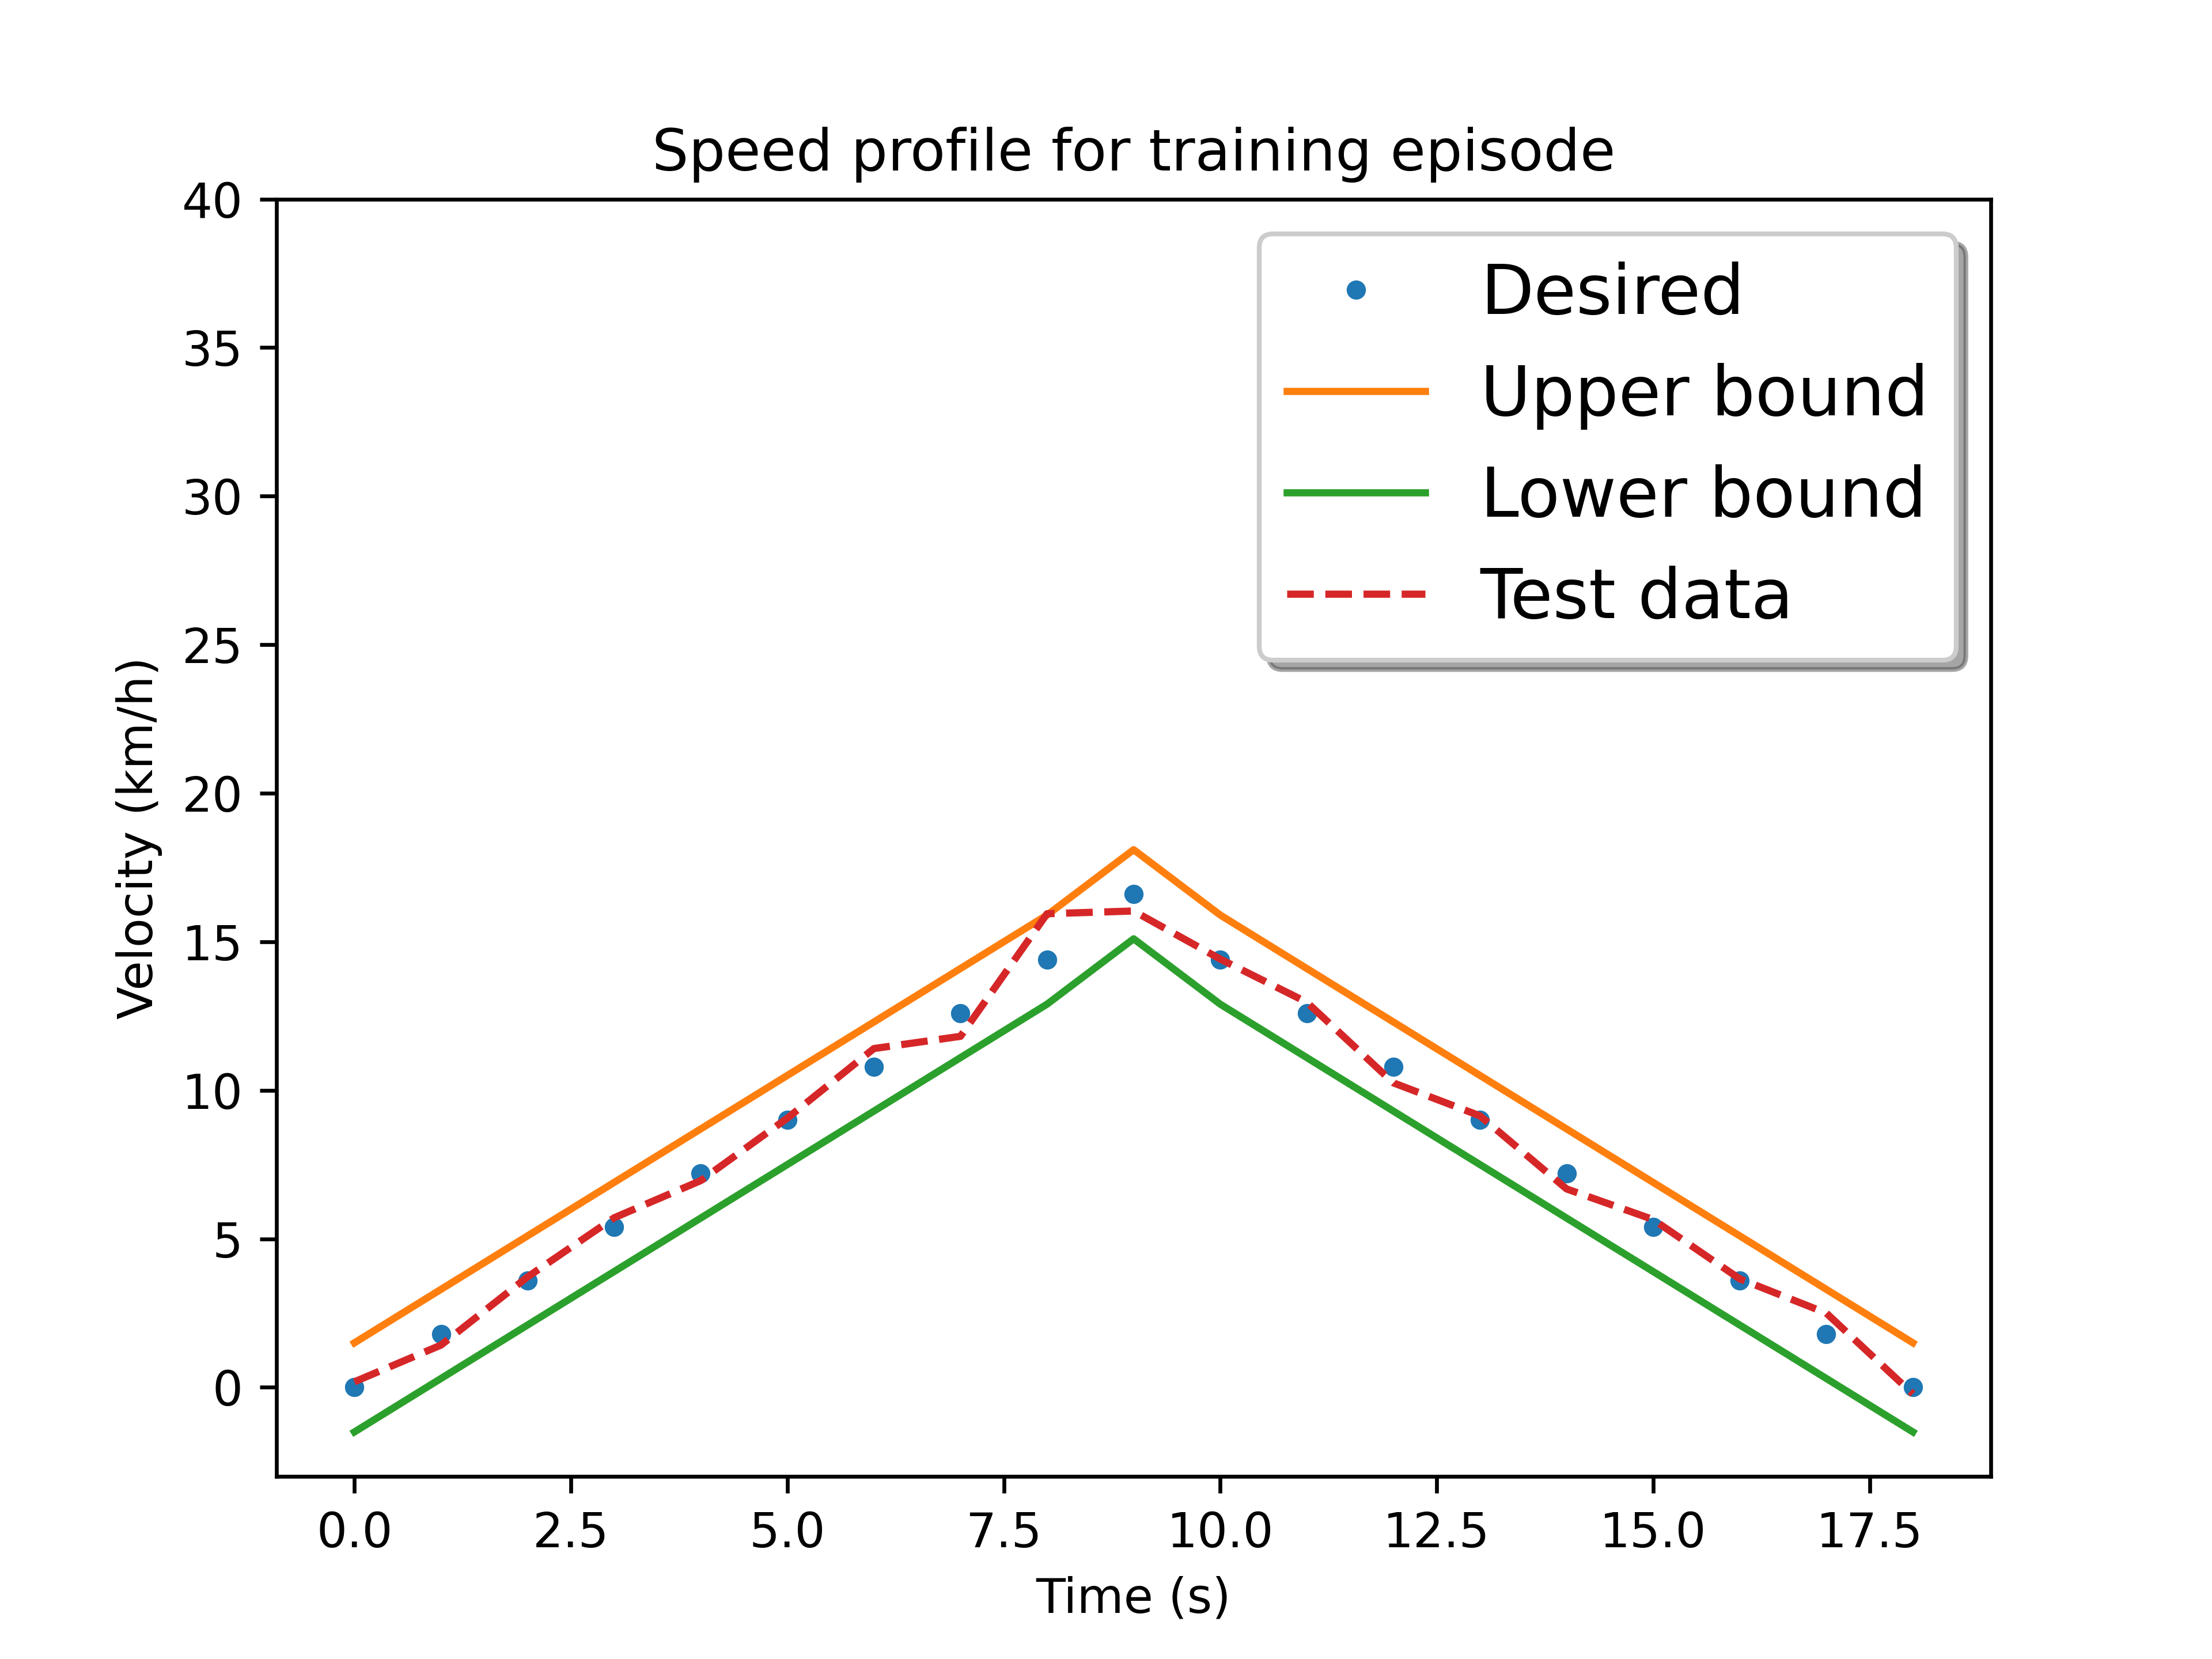
\includegraphics[scale=0.5]{images/speed_profile.png}
		\captionof{figure}{\label{fig:speed profile for traning} Speed profile of the episode used for training}
	\end{minipage}
\end{figure}

\begin{description}
	\item[State] at timestamp $t$ is denoted by $s_t$
	      \begin{itemize}
		      \item $v_k$: velocity of the vehicle
		      \item $a_k$: acceleration pedal position in percentage
		      \item $b_k$: brake pedal position in percentage
		      \item $k$: number of frames within a single record. a record starts from timestamp $t$, contains $k$ can frames and ends by the end of the last frame
		      \item each line in a record is referred to as a single frame, whose information can be extracted from multiple can frames at the same moment
		      \item rows within a record is contiguous in time starting from the timestamp $t$
		      \item in case of frame loss, a loss token needs to be inserted as a lost frame state at the next timestamp of $t$, that is $t+1$
	      \end{itemize}
	\item[Next State] the next state following $s_t$ is denoted by $s'_t$
	      \begin{itemize}
		      \item the state according to which the next decsion $a_t$ will be made.
		      \item in case of previous assumption, this state will contain the next adjacent 30 frames of state $s_t$.
		      \item $s'_t$ must be contiguous in time to $s_t$
	      \end{itemize}
	\item[Action] at timestamp $t$ is denoted by $a_t$
	      \begin{itemize}
		      \item it's the decision of what pedal map will be applied after observing the state $s_t$ by the agent
		      \item the action $a_t$ of veos system is the pedal map $[pm_{5\times17}]^t$ at timestamp $t$. it's currently 5 consecutive rows in the full pedal map corresponding to the current state $s_t$, 17 is the current discretization level of the throttle pedal percentage. each element of the pedal map is the requested torque given the vehicle velocity and the throttle pedal position
		      \item the real effective time of $a_t$ could be delayed by $\delta t$ due to transmission and flashing latency, i.e. $a_t$ will be applied at $t+\delta t$
		      \item $a_t$ must precede $s'_t$, that is $t+\delta t < t+1$ so that the next state $s'_t$ is the result of applying $a_t$
	      \end{itemize}
	\item[Reward] at timestamp $t$ is denoted by $r_t$
	      \begin{itemize}
		      \item it's the electricity consumption effected by the action $a_t$
		      \item it's computed by accumlating the product of battery voltage $u_{r_k}$ and current values $i_{r_k}$ at the frames after the current action $a_t$ is applied and before the next action $a_{t+1}$ becomes effective, that is to say, the voltage and current values after the moment $r_0$  when flashi1ng the pedal map is done and in effect, until after the last effective moment $r_k$  when the next action $a_{t+1}$ is applied (flashed and in effect)
	      \end{itemize}
	\item[Record] is the uploading unit of remote-can module. Tt's a timestamped quadruple, which is a tuple of 4 elements $(s_t, a_t, r_t, s'_t)$ with a timestamp $t$
	      \begin{itemize}
		      \item a record without timestamp is called a quadruple
		      \item the sequence of records consist of an episode
	      \end{itemize}
	\item[Episode] An episode is a consecutive sequence of Record with a start and a termination state which typically represents a driving route/task or a test case and the vehicle operates on routinely.
	      \begin{itemize}
		      \item *Triple*: Since the sequence is consecutive, the next state $s'_t$ is the next adjacent state $s_{t+1}$ and thus not required in the tuple. Therefore one record is reduced to a triple.
		      \item *Null elements*: Care needs to be taken to insert null elements in the sequence in case of absent records.
		      \item *Ragged*: $T$ is the total time steps of the episode. Episodes have different sequence length, since the termination of an episode could mean reaching the destination with different speeds or events. Therefore the episode pool  is ususally ragged.
		      \item $e_T=[(s_0,a_0,r_0),(s_1,a_1,r_1), \ldots,(s_{T-1},a_{T-1},r_{T-1})]$
	      \end{itemize}
\end{description}

The structure of the record looks like the following table


each driver has his own driving style which we model as part of the whole environment.

we can collect a huge amount of drivng data (acceleration pedal, brake pedal, the resulting speed, the energy consumption, the voltage and the current from electric powertain), due to its low data density. we can record and process a long period of driving, to figure out a long-term optimal driving policy regards to what is an energy efficient way of driving.


We cannot leverage simulation, because there's no efficient simulation available for electric powertrain and complex road condition. Part of the reason is that modeling the real road condition and electric motor is very difficult.

in low speed, there's a coast-down profile which keeps the vehicle in moving forward in low speed
\section{system design}
\label{sec:design}




A new real world application of deep reinforcement learning, with considerations of leveraging capacity of deep neural network to make use of a large mount of data.

checking and review the applications of current deep rl techniques, in theory and practice. Caveats regarding the issues of applying deep reinforcement. System design and experiment design, data collection, safety, system resi
interesting issues of system safety and persistance, task persistance.
explore the application of recent offline-reinforcment learning in this application.

\begin{figure}[ht]
	\centering
	\def\svgwidth{0.8\columnwidth}
	\input{images/veos_system.pdf_tex}
	\caption{\label{fig:veos} EVEOS system}
	\label{fig:EVEOS system}
\end{figure}


%\begin{figure}[ht]
%	\centering
%	\begin{subfigure}[b]{0.45\textwidth}
%		\centering
%		\def\svgwidth{\columnwidth}
%		\input{images/veos_system.pdf_tex}
%		\caption{\label{fig:veos} EVEOS system}
%		\label{fig:EVEOS system}
%	\end{subfigure}
%	\hfill
%	\begin{subfigure}[b]{0.45\textwidth}
%		\centering
%		\def\svgwidth{\columnwidth}
%		% Data flow diagram
% Author: David Fokkema
\documentclass{standalone}
\usepackage{tikz}
\usetikzlibrary{arrows,quotes,shapes.multipart,arrows.meta,matrix,shapes.geometric,backgrounds}

% Defines a `datastore' shape for use in DFDs.  This inherits from a
% rectangle and only draws two horizontal lines.
\makeatletter
\pgfdeclareshape{datastore}{
  \inheritsavedanchors[from=rectangle]
  \inheritanchorborder[from=rectangle]
  \inheritanchor[from=rectangle]{center}
  \inheritanchor[from=rectangle]{base}
  \inheritanchor[from=rectangle]{north}
  \inheritanchor[from=rectangle]{north east}
  \inheritanchor[from=rectangle]{east}
  \inheritanchor[from=rectangle]{south east}
  \inheritanchor[from=rectangle]{south}
  \inheritanchor[from=rectangle]{south west}
  \inheritanchor[from=rectangle]{west}
  \inheritanchor[from=rectangle]{north west}
  \backgroundpath{
    %  store lower right in xa/ya and upper right in xb/yb
    \pgfset{outer xsep=1.5cm}
    \pgfset{outer ysep=1.5cm}
    \southwest \pgf@xa=\pgf@x \pgf@ya=\pgf@y
    \northeast \pgf@xb=\pgf@x \pgf@yb=\pgf@y
    \pgfpathmoveto{\pgfpoint{\pgf@xa}{\pgf@ya}}
    \pgfpathlineto{\pgfpoint{\pgf@xb}{\pgf@ya}}
    \pgfpathmoveto{\pgfpoint{\pgf@xa}{\pgf@yb}}
    \pgfpathlineto{\pgfpoint{\pgf@xb}{\pgf@yb}}
 }
}
\makeatother

\tikzset{
  database_plate/.style={
    cylinder,draw,rotate=90,minimum width=1.5cm,path picture=
    {
      \draw (path picture bounding box.160) to[out=180,in=180,looseness=0.3] (path picture bounding box.20);
      \draw (path picture bounding box.200) to[out=180,in=180,looseness=0.3] (path picture bounding box.340);
    }
  },
  database/.style={
    cylinder,shading=axis,shading angle=0,top color=yellow!10,bottom color=yellow!60,draw,rotate=90,minimum width=1.5cm
  }
}

\begin{document}
\begin{tikzpicture}[
  font=\sffamily,
  every matrix/.style={ampersand replacement=\&,column sep=2cm,row sep=2cm},
  hw/.style={draw,thick,minimum width=2cm,minimum height=1cm,rounded corners,fill=yellow!20,inner sep=.3cm},
  process/.style={draw,thick,circle,fill=blue!20},
  multimodal/.style={circle split,draw,double,fill=blue!20,font=\sffamily\tiny},
  sink/.style={hw,fill=green!20},
  datastore/.style={draw,very thick,shape=datastore,inner sep=.3cm},
  dots/.style={gray,scale=2},
  to/.style={->,>=stealth',shorten >=1pt,semithick,font=\sffamily\footnotesize},
  every edge/.style={draw,>=stealth,shorten <=1pt, shorten >=1pt,semithick,font=\sffamily\footnotesize},
  every edge quotes/.style={auto=left,sloped,font=\sffamily\small},
  every node/.style={align=center}
]
  %every edge/.style={->,>=stealth',shorten >=1pt,semithick,font=\sffamily\footnotesize},
  % Fill the background


  % Position the nodes using a matrix layout
  \matrix (m) [matrix of nodes,
      row sep = 2em, column sep = 2em,
      minimum size=2cm]{
    |[multimodal,rotate=90] (cl)| {
      Cloud OSS \nodepart{lower}
    } RemoteCAN
    \& |[database] (db)| {Storage}
    \& |[process] (mo)| {Model} \\
    |[process] (av)| {Avatar}
    \& |[process] (cr)| {Cruncher}
    \& |[process] (ag)| {Agent} \\
    |[multimodal] (kv)| {
      KvaserCAN
      \nodepart{lower}
    } CAN/UDP server
    \&
    \& \\
    |[hw] (v)| {ECU} \&  \&\\
  };

  % Draw the arrows between the nodes and label them.
  \draw (cr.2) edge [arrows={-Stealth[harpoon]},"observation\\\texttt{\string[Dataframe\string]}",midway,align=center] (ag.178)
        (ag.182) edge [arrows={-Stealth[harpoon]},"\texttt{\string[Dataframe\string]}\\action"',midway,align=center] (cr.358);
  \draw (kv.47) edge [arrows={-Stealth[harpoon]},"Pipeline\\\texttt{\string[json/Dataframe\string]}",midway,align=center] (cr.223)
        (cr.227) edge [arrows={-Stealth[harpoon]},"\texttt{\string[Dataframe/json\string]}\\Pipeline"',midway,align=center] (kv.43);
  \draw (cl.227) edge [arrows={-Stealth[harpoon]},"Pipeline\\\texttt{\string[json/Dataframe\string]}",midway,align=center] (cr.133)
        (cr.137) edge [arrows={-Stealth[harpoon]},"\texttt{\string[Dataframe/json\string]}\\Pipeline"',midway,align=center] (cl.223);
  \draw (db.227) edge [arrows={-Stealth[harpoon]},"Batches\\\texttt{\string[Dataframe\string]}",midway,align=center] (ag.133)
        (ag.137) edge [arrows={-Stealth[harpoon]},"\texttt{\string[Dataframe\string]}\\Episode"',midway,align=center,pos=0.6] (db.223);
  \draw (ag.92) edge [arrows={-Stealth[harpoon]},"observation\\\texttt{\string[Dataframe\string]}",midway,align=center] (mo.268)
        (mo.272) edge [arrows={-Stealth[harpoon]},"action\\\texttt{\string[Dataframe\string]}",midway,align=center] (ag.88);
  \draw (ag.0) edge [->,bend right,"\texttt{\string[Dataframe\string]}\\Batches"',midway,align=center] (mo.0);
  \draw (mo) edge[->,loop left,out=225,in=135, looseness=5] node[font=\sffamily\small,right]{Train} (mo);
  \draw (av.2) edge [->,dotted,"config." above,"sched." below,font=\sffamily\tiny] (cr.178);
  \draw (kv) edge [<-,dotted,"config." above,"sched." below,font=\sffamily\tiny] (av);
  \draw (av) edge [->,dotted,"config." above,"sched." below,font=\sffamily\tiny] (cl);
  \draw (v) edge [<->,"CAN" above, "UDP" below] (kv);
  \draw (cl.137) edge [<->, densely dash dot dot,bend right,"OTA"] node[hw,minimum width=1cm,minimum height=0.5cm,solid,very near end, sloped,]{TBox} (v.133);

  % Background rectangle
    \begin{scope}[on background layer]
        \fill[green!10] (current bounding box.south west) rectangle (current bounding box.north east);
    \end{scope}
\end{tikzpicture}
\end{document}

%		\caption{\label{fig:label} Software Overview}
%		\label{fig:tspace}
%	\end{subfigure}
%\end{figure}


\subsection{Data pipelines}

\begin{figure}[ht]
	\centering
	\def\svgwidth{0.8\columnwidth}
	% Data flow diagram
% Author: David Fokkema
\documentclass{standalone}
\usepackage{tikz}
\usetikzlibrary{arrows,quotes,shapes.multipart,arrows.meta,matrix,shapes.geometric,backgrounds}

% Defines a `datastore' shape for use in DFDs.  This inherits from a
% rectangle and only draws two horizontal lines.
\makeatletter
\pgfdeclareshape{datastore}{
  \inheritsavedanchors[from=rectangle]
  \inheritanchorborder[from=rectangle]
  \inheritanchor[from=rectangle]{center}
  \inheritanchor[from=rectangle]{base}
  \inheritanchor[from=rectangle]{north}
  \inheritanchor[from=rectangle]{north east}
  \inheritanchor[from=rectangle]{east}
  \inheritanchor[from=rectangle]{south east}
  \inheritanchor[from=rectangle]{south}
  \inheritanchor[from=rectangle]{south west}
  \inheritanchor[from=rectangle]{west}
  \inheritanchor[from=rectangle]{north west}
  \backgroundpath{
    %  store lower right in xa/ya and upper right in xb/yb
    \pgfset{outer xsep=1.5cm}
    \pgfset{outer ysep=1.5cm}
    \southwest \pgf@xa=\pgf@x \pgf@ya=\pgf@y
    \northeast \pgf@xb=\pgf@x \pgf@yb=\pgf@y
    \pgfpathmoveto{\pgfpoint{\pgf@xa}{\pgf@ya}}
    \pgfpathlineto{\pgfpoint{\pgf@xb}{\pgf@ya}}
    \pgfpathmoveto{\pgfpoint{\pgf@xa}{\pgf@yb}}
    \pgfpathlineto{\pgfpoint{\pgf@xb}{\pgf@yb}}
 }
}
\makeatother

\tikzset{
  database_plate/.style={
    cylinder,draw,rotate=90,minimum width=1.5cm,path picture=
    {
      \draw (path picture bounding box.160) to[out=180,in=180,looseness=0.3] (path picture bounding box.20);
      \draw (path picture bounding box.200) to[out=180,in=180,looseness=0.3] (path picture bounding box.340);
    }
  },
  database/.style={
    cylinder,shading=axis,shading angle=0,top color=yellow!10,bottom color=yellow!60,draw,rotate=90,minimum width=1.5cm
  }
}

\begin{document}
\begin{tikzpicture}[
  font=\sffamily,
  every matrix/.style={ampersand replacement=\&,column sep=2cm,row sep=2cm},
  hw/.style={draw,thick,minimum width=2cm,minimum height=1cm,rounded corners,fill=yellow!20,inner sep=.3cm},
  process/.style={draw,thick,circle,fill=blue!20},
  multimodal/.style={circle split,draw,double,fill=blue!20,font=\sffamily\tiny},
  sink/.style={hw,fill=green!20},
  datastore/.style={draw,very thick,shape=datastore,inner sep=.3cm},
  dots/.style={gray,scale=2},
  to/.style={->,>=stealth',shorten >=1pt,semithick,font=\sffamily\footnotesize},
  every edge/.style={draw,>=stealth,shorten <=1pt, shorten >=1pt,semithick,font=\sffamily\footnotesize},
  every edge quotes/.style={auto=left,sloped,font=\sffamily\small},
  every node/.style={align=center}
]
  %every edge/.style={->,>=stealth',shorten >=1pt,semithick,font=\sffamily\footnotesize},
  % Fill the background


  % Position the nodes using a matrix layout
  \matrix (m) [matrix of nodes,
      row sep = 2em, column sep = 2em,
      minimum size=2cm]{
    |[multimodal,rotate=90] (cl)| {
      Cloud OSS \nodepart{lower}
    } RemoteCAN
    \& |[database] (db)| {Storage}
    \& |[process] (mo)| {Model} \\
    |[process] (av)| {Avatar}
    \& |[process] (cr)| {Cruncher}
    \& |[process] (ag)| {Agent} \\
    |[multimodal] (kv)| {
      KvaserCAN
      \nodepart{lower}
    } CAN/UDP server
    \&
    \& \\
    |[hw] (v)| {ECU} \&  \&\\
  };

  % Draw the arrows between the nodes and label them.
  \draw (cr.2) edge [arrows={-Stealth[harpoon]},"observation\\\texttt{\string[Dataframe\string]}",midway,align=center] (ag.178)
        (ag.182) edge [arrows={-Stealth[harpoon]},"\texttt{\string[Dataframe\string]}\\action"',midway,align=center] (cr.358);
  \draw (kv.47) edge [arrows={-Stealth[harpoon]},"Pipeline\\\texttt{\string[json/Dataframe\string]}",midway,align=center] (cr.223)
        (cr.227) edge [arrows={-Stealth[harpoon]},"\texttt{\string[Dataframe/json\string]}\\Pipeline"',midway,align=center] (kv.43);
  \draw (cl.227) edge [arrows={-Stealth[harpoon]},"Pipeline\\\texttt{\string[json/Dataframe\string]}",midway,align=center] (cr.133)
        (cr.137) edge [arrows={-Stealth[harpoon]},"\texttt{\string[Dataframe/json\string]}\\Pipeline"',midway,align=center] (cl.223);
  \draw (db.227) edge [arrows={-Stealth[harpoon]},"Batches\\\texttt{\string[Dataframe\string]}",midway,align=center] (ag.133)
        (ag.137) edge [arrows={-Stealth[harpoon]},"\texttt{\string[Dataframe\string]}\\Episode"',midway,align=center,pos=0.6] (db.223);
  \draw (ag.92) edge [arrows={-Stealth[harpoon]},"observation\\\texttt{\string[Dataframe\string]}",midway,align=center] (mo.268)
        (mo.272) edge [arrows={-Stealth[harpoon]},"action\\\texttt{\string[Dataframe\string]}",midway,align=center] (ag.88);
  \draw (ag.0) edge [->,bend right,"\texttt{\string[Dataframe\string]}\\Batches"',midway,align=center] (mo.0);
  \draw (mo) edge[->,loop left,out=225,in=135, looseness=5] node[font=\sffamily\small,right]{Train} (mo);
  \draw (av.2) edge [->,dotted,"config." above,"sched." below,font=\sffamily\tiny] (cr.178);
  \draw (kv) edge [<-,dotted,"config." above,"sched." below,font=\sffamily\tiny] (av);
  \draw (av) edge [->,dotted,"config." above,"sched." below,font=\sffamily\tiny] (cl);
  \draw (v) edge [<->,"CAN" above, "UDP" below] (kv);
  \draw (cl.137) edge [<->, densely dash dot dot,bend right,"OTA"] node[hw,minimum width=1cm,minimum height=0.5cm,solid,very near end, sloped,]{TBox} (v.133);

  % Background rectangle
    \begin{scope}[on background layer]
        \fill[green!10] (current bounding box.south west) rectangle (current bounding box.north east);
    \end{scope}
\end{tikzpicture}
\end{document}

	\caption{\label{fig:label} Software Overview}
\end{figure}


\section{Result and discussion}
\label{sec:result}


\section{Conclusion}
\label{sec:conclusion}

\begin{appendices}
	\section{dataflow}
	The dataflow of the pipelines
	\section{MLOps}
	The ML operations
\end{appendices}
%\bibliographystyle{unsrtnat}
%\bibliographystyle{abbrvnat}
%%% Uncomment this section and comment out the \bibliography{references} line above to use inline references.
% \begin{thebibliography}{1}

% 	\bibitem{kour2014real}
% 	George Kour and Raid Saabne.
% 	\newblock Real-time segmentation of on-line handwritten arabic script.
% 	\newblock In {\em Frontiers in Handwriting Recognition (ICFHR), 2014 14th
% 			International Conference on}, pages 417--422. IEEE, 2014.

% 	\bibitem{kour2014fast}
% 	George Kour and Raid Saabne.
% 	\newblock Fast classification of handwritten on-line arabic characters.
% 	\newblock In {\em Soft Computing and Pattern Recognition (SoCPaR), 2014 6th
% 			International Conference of}, pages 312--318. IEEE, 2014.

% 	\bibitem{keshet2016prediction}
% 	Keshet, Renato, Alina Maor, and George Kour.
% 	\newblock Prediction-Based, Prioritized Market-Share Insight Extraction.
% 	\newblock In {\em Advanced Data Mining and Applications (ADMA), 2016 12th International
%                       Conference of}, pages 81--94,2016.

% \end{thebibliography}

\printbibliography

\end{document}
